\documentclass[parskip=full]{scrartcl}
\usepackage[utf8]{inputenc} % use utf8 file encoding for TeX sources
\usepackage[T1]{fontenc}    % avoid garbled Unicode text in pdf
\usepackage[german]{babel}  % german hyphenation, quotes, etc
\usepackage{graphicx}
\usepackage{rotating}
\graphicspath{ {images/} }
\usepackage{hyperref}       % detailed hyperlink/pdf configuration
\hypersetup{                % ‘texdoc hyperref‘ for options
pdftitle={PSE : DataMovementDeaon},%
bookmarks=true,%
}
\usepackage{graphicx}       % provides commands for including figures
\usepackage{csquotes}       % provides \enquote{} macro for "quotes"
\usepackage[nonumberlist, acronym]{glossaries} % provides glossary commands
\usepackage{enumitem}
\usepackage{lscape}
\usepackage{caption}
\usepackage{rotating}
\usepackage{placeins}

\makenoidxglossaries
%
%%Glossary
%

\begin{document}

\begin{titlepage}
\centering
{\scshape\LARGE Karlsruher Institut für Technologie\par}
\vspace{1cm}
{\scshape\Large Functional Specification Document (FSD)\par}
\vspace{1.5cm}
{\huge\bfseries Numerical Linear Algebra meets Machine Learning \par}
\vspace {2cm}

{\Large\itshape Fabian Koffer\par}
{\Large\itshape Simon Hanselmann\par}
{\Large\itshape Yannick Funk\par}
{\Large\itshape Dennis Leon Gr\"{o}tzinger\par}
{\Large\itshape Anna Katharina Ricker\par}

\vfill
Supervisors\par
Hartwig Anzt
Makus G\"{o}tz

\vfill
{\large\today\par}
\end{titlepage}



\section{Success Criteria}

Goal is the delivery of a consistent software stack that allows for employing 
neural networks for the linear system classification. 
The ecosystem should allow to train a neural network on selecting a suitable iterative solver depending on the linear system characteristics.

\subsection{Mandatory Requirements}
\begin{itemize}

\item A software that supports the described work-flow design including the embedding of external components.

\item The software must be cross-platform compatible and support at least a Linux and the Windows operating system.

\item The software must be usable via a command-line interface (CLI).

\item A data exchange format design that allows to store matrices and annotate them with 
additional meta-data, including labels.

\item An extensible design for multiple entities that are able to generate matrices in the proposed exchange format.

\item There need to be two actual realizations of these entities, which:

\begin{itemize}
    \item allow to generate artificial noise with uniform and gaussian noise as well as
    
    \item can fetch test matrices from the Suite Sparse matrix collection.
\end{itemize}

\item A dataset of at least 500 matrices in the envisioned data format and generated by the above two entities. There smallest share of matrices of a given entity must be no less than 30\% of the total number of contained matrices.

\item An extensible design that allows to solve the matrices using a configurable set of iterative solver algorithms using a newly developed binding to the Ginkgo linear algebra library.

\item A readily implemented and trained neural network of the ResNet architecture. It must be able to predict for a given matrix (in arbitrary format), which of the iterative solver algorithms is the most suitable.

\item An entity that allows to store and load the trained neural network.

\item The software must include entities for training and re-training a neural network from scratch, respectively from a previously stored state.

\item The software must be able to show the predicted algorithm and its associated suitability probability on the standard output.

\item Realization of a sustainable and quality-assured software development process. This includes a software design document, in-code documentation, unit testing and a continuous integration (CI).

\end{itemize}

\subsection{Optional Requirements}

\begin{itemize}
    
\item Scalability of the work-flow including matrix generation, training, prediction in that multiple processors may be used in parallel.

\item The software must be able to utilize GPU accelerators for the training and prediction capabilities of the neural network.

\item The system must support at least five iterative solver algorithms.

\item A web interface to the software that is able to select a single, a set or all matrices of an uploadable file for prediction by the neural network. The web interface may also be able to visualize the contained matrices, annotated labels as well as prediction results.

\end{itemize}

\subsection{demarcation criteria}

\section{Product use}
\subsection{Scope of application}
The software will be used for scientific work in the field of math and computer science.
\subsection{Target groups}
Mathematican and computer scientists who are working with sparse linear systems.
\subsection{Operating conditions}

\begin{itemize}
\item Use in the field of scientific work
\item Office environment
\end{itemize}

\section{Product enviroment}


\subsection{Software}

\begin{itemize}
\item The product will run on Windows 10 and Linux distributions 
\item The labeling of the matricies and training of the neural network will be done with Linux
\end{itemize}

\subsection{Hardware}

\begin{itemize}
\item The product will run on a workstation computer
\item The labeling of the matricies and training of the neural network will be done on a server with multiple GPUs
\end{itemize}

\subsection{Orgware}
A Documentation for the user will be generated.


\section{Functional requirements}
\subsection{Artificial matrix generator}
\subsection{Matrix label}
\subsection{Matrix train and test}
\subsection{Matrix classification }

\section{Product data}
\begin{itemize}
\item 500-1000 matrices for training, validation and test
\end{itemize}

\section{Nonfunctional requirements}

\section{Global test cases}
\subsection{the following function sequences must be checked}
\subsection{the following data consistencies must be checked}
\newpage
\section{System models}
\subsection{Scenarios}
\subsubsection{User}
\begin{samepage} 
The User safes the sparse linear matrix in any desired filepath. Afterwards the user starts our program. The command open <filepath> loads the matrix in the program. That is when the neural network will classify the matrix and determine the fastest iterative solver/preconditioner combination for solving the matrix. This combination will be printed to the command line. (\textbf{Optional:} After determining the fastest combination the program will solve the matrix with this combination. The solved matrix will be safed in a directory the user specifies.)
 \end{samepage}
\subsection{Use cases}
\subsection{Object models}
\subsection{dynamic models}
\subsection{Command line options}

\subsection{Use of the classifier}
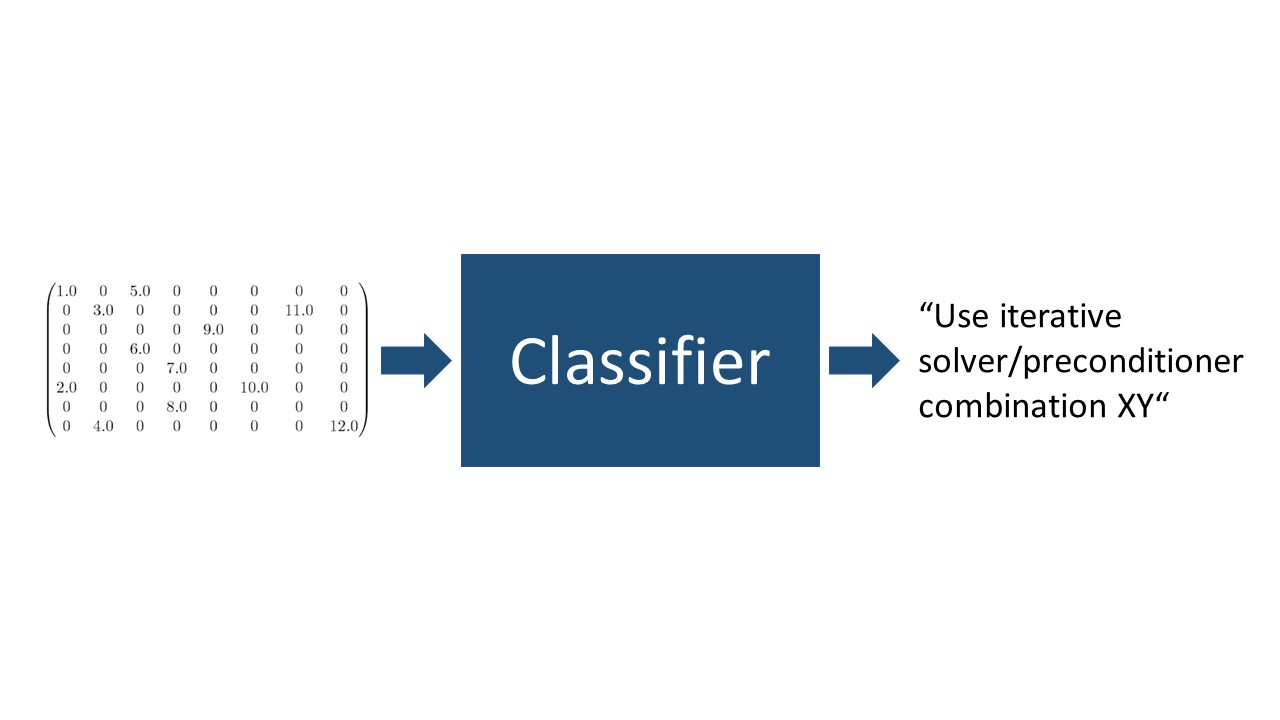
\includegraphics[scale=0.6, angle=90]{ClassifierUse}

\subsection{Workflow}
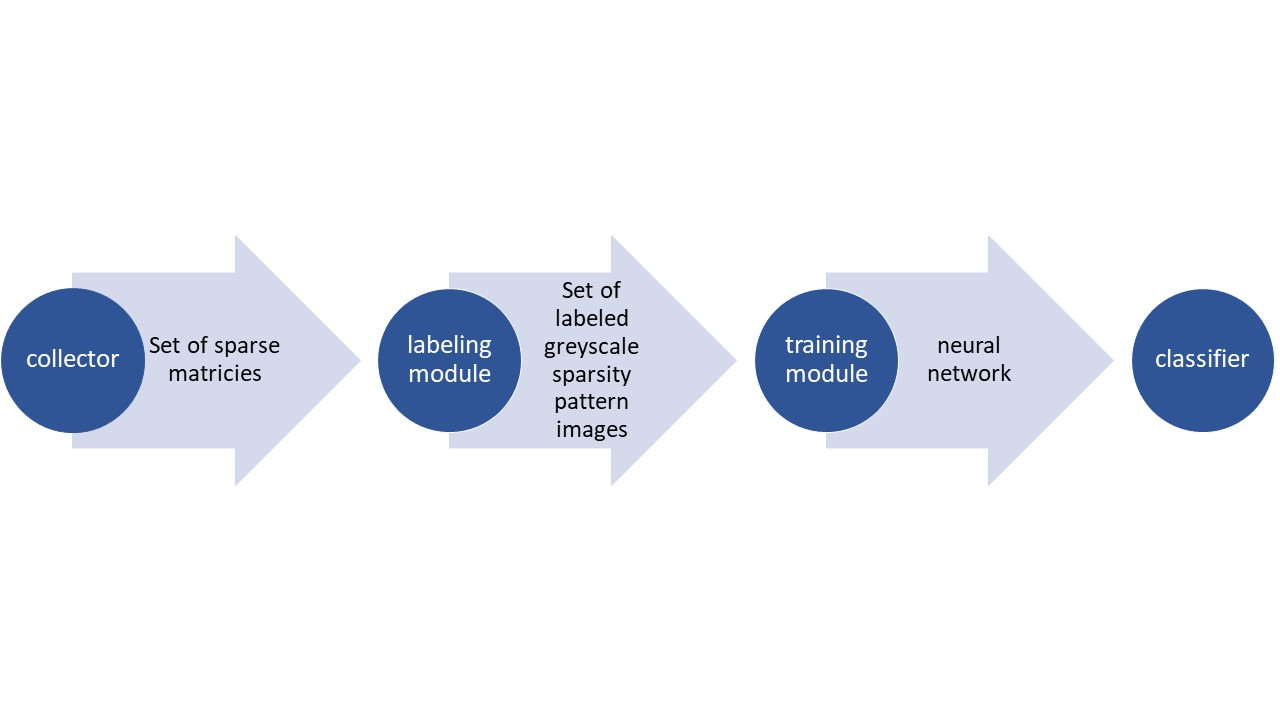
\includegraphics[scale=0.5, angle=90]{workflow}
\section{Glossar}

% % Automatisch generiertes Glossar (Latex zwei mal ausführen um Glossar anzuzeigen)
%
%\glsaddall % das sorgt dafür, dass alles Glossareinträge gedruckt werden, nicht nur die verwendeten. Das sollte nicht nötig sein!
\printnoidxglossaries

\end{document}